\documentclass{article}

% content/resources/templates/preamble.tex
\usepackage[margin=0.6in]{geometry}
\author{Milav Dabgar}
\usepackage{amsmath,amssymb,amsthm}
\usepackage{booktabs}
\usepackage{multirow}
\usepackage{xcolor}
\usepackage{tcolorbox}
\tcbuselibrary{breakable,skins}
\usepackage[colorlinks=true,linkcolor=blue]{hyperref}
\usepackage{titlesec}
\usepackage{enumitem}
\usepackage{tikz}
\usepackage{pgfplots}
\usepackage{circuitikz}
\usepackage[version=4]{mhchem}
\usepackage{longtable}
\usepackage{array}
\usepackage{float}
\usepackage{caption}
\usepackage{listings}

\lstset{
  basicstyle=\small\ttfamily,
  breaklines=true,
  breakatwhitespace=false,
  postbreak=\mbox{\textcolor{red}{$\hookrightarrow$}\space},
  float=false,
  numbers=left,
  numberstyle=\tiny\color{gray},
  numbersep=10pt,
  xleftmargin=2em,
  keywordstyle=\color{blue},
  commentstyle=\color{green!60!black},
  stringstyle=\color{purple},
  backgroundcolor=\color{gray!5},
  showstringspaces=false,
  tabsize=2,
  captionpos=b,
  keepspaces=true,
  columns=flexible
}

\pgfplotsset{compat=1.18}
\usetikzlibrary{shapes,arrows,positioning,calc,patterns,decorations.pathmorphing,decorations.markings,arrows.meta}

% Color scheme
\definecolor{headcolor}{RGB}{0,102,204}
\definecolor{keycolor}{RGB}{220,20,60}
\definecolor{solutioncolor}{RGB}{34,139,34}
\definecolor{mnemoniccolor}{RGB}{148,0,211}
\definecolor{codecolor}{RGB}{0,0,100}

% Spacing
\setlength{\parskip}{3pt}
\setlist[itemize]{nosep}
\setlist[enumerate]{nosep}

% Title formatting
\titleformat{\section}{\Large\bfseries\color{headcolor}}{\thesection}{1em}{}
\titleformat{\subsection}{\large\bfseries\color{headcolor}}{\thesubsection}{1em}{}

% Pandoc tightlist compatibility
\providecommand{\tightlist}{%
  \setlength{\itemsep}{0pt}\setlength{\parskip}{0pt}}

% Pandoc longtable compatibility
\newcounter{none}
\def\thenone{}


% content/resources/templates/english-boxes.tex

% Custom environments
\newtcolorbox{solutionbox}{
 breakable,
 enhanced,
 colback=solutioncolor!5!white,
 colframe=solutioncolor!75!black,
 fonttitle=\bfseries,
 title=Solution
}

\newtcolorbox{solutionboxnobreak}{
 colback=solutioncolor!5!white,
 colframe=solutioncolor!75!black,
 fonttitle=\bfseries,
 title=Solution
}

\newtcolorbox{keyformula}{
 breakable,
 enhanced,
 colback=keycolor!5!white,
 colframe=keycolor!75!black,
 fonttitle=\bfseries,
 title=Key Formula
}

\newtcolorbox{mnemonicboxenv}{
 breakable,
 enhanced,
 colback=mnemoniccolor!5!white,
 colframe=mnemoniccolor!75!black,
 fonttitle=\bfseries,
 title=Mnemonic
}

\newcommand{\mnemonicbox}[1]{%
  \begin{mnemonicboxenv}
    #1
  \end{mnemonicboxenv}
}


% Custom commands for GTU solutions
% This file defines semantic commands for consistent formatting

% Question command with automatic formatting
\newcommand{\question}[2]{%
  \section*{Question #1}%
  \textbf{#2}%
}

% OR question variant
\newcommand{\questionor}[2]{%
  \section*{Question #1 OR}%
  \textbf{#2}%
}

% Proper table environment with caption
\newenvironment{answertable}[1]{%
  \begin{table}[htbp]
  \centering
  \caption{#1}
}{%
  \end{table}
}

% Proper figure environment for diagrams
\newenvironment{answerdiagram}[1]{%
  \begin{figure}[htbp]
  \centering
  \caption{#1}
}{%
  \end{figure}
}

% Semantic markup for key terms
\newcommand{\keyword}[1]{\textbf{#1}}
\newcommand{\code}[1]{\texttt{#1}}
\newcommand{\classname}[1]{\texttt{#1}}
\newcommand{\methodname}[1]{\texttt{#1}}

% Proper quotation marks
\newcommand{\mnemonic}[1]{``#1''}


\title{Electronic Circuits \& Applications (4321103) - Winter 2024 Solution}
\date{January 13, 2024}

\begin{document}
\maketitle

\questionmarks{1}{a}{3}
\textbf{Explain amplifier parameters Ai, Ri and Ro for CE configuration.}

\begin{solutionbox}
\textbf{CE Amplifier Parameters:}

\begin{center}
\captionof{table}{CE Amplifier Parameters}
\begin{tabular}{|l|l|l|}
\hline
\textbf{Parameter} & \textbf{Definition} & \textbf{value} \\ \hline
Current Gain ($A_i$) & Ratio of output current to input current & High (20-500) \\ \hline
Input Resistance ($R_i$) & Opposition to current flow at input & Medium (1-2 k$\Omega$) \\ \hline
Output Resistance ($R_o$) & Opposition to current flow at output & High (40-50 k$\Omega$) \\ \hline
\end{tabular}
\end{center}

\begin{center}
\begin{tikzpicture}[node distance=2.5cm, auto]
    \node [gtu block] (amp) {CE Amplifier};
    \node [left of=amp, node distance=3cm] (in) {Input};
    \node [right of=amp, node distance=3cm] (out) {Output};
    
    \draw [gtu arrow] (in) -- node[above] {$R_i$: 1-2 k$\Omega$} (amp);
    \draw [gtu arrow] (amp) -- node[above] {$A_i$: 20-500} (out);
    \draw [gtu arrow] (amp) -- node[below] {$R_o$: 40-50 k$\Omega$} (out);
\end{tikzpicture}
\end{center}
\end{solutionbox}
\begin{mnemonicbox}
CAR - CE has Current gain high, Average input resistance, and Robust output resistance.
\end{mnemonicbox}

\questionmarks{1}{b}{4}
\textbf{Write short-note on heat sink.}

\begin{solutionbox}
\textbf{Heat Sink:}
A device that absorbs and dissipates heat from electronic components to prevent overheating.

\begin{center}
\begin{tikzpicture}[node distance=2.5cm, auto]
    \node [gtu block] (T) {Transistor};
    \node [gtu block, right of=T] (HS) {Heat Sink};
    \node [right of=HS, node distance=3cm] (Air) {Ambient Air};

    \draw [gtu arrow] (T) -- (HS);
    \draw [gtu arrow] (HS) -- node[above] {Heat Dissipation} (Air);

    % Structure visual
    \node [draw, fill=gray!20, minimum height=1cm, minimum width=0.2cm, below of=HS, node distance=1.5cm] (Base) {};
    \foreach \x in {-0.4, -0.2, 0, 0.2, 0.4}
        \draw (Base.east) ++(0, \x) -- ++(0.5, 0);
    \node [right of=Base, node distance=1cm] {Fins};
\end{tikzpicture}
\end{center}

\textbf{Types of Heat Sinks:}
\begin{itemize}
    \item \textbf{Passive}: Rely on natural convection (no fans).
    \item \textbf{Active}: Use fans for forced air convection.
    \item \textbf{Liquid-cooled}: Use liquid for better heat transfer.
\end{itemize}

\textbf{Key Functions:}
\begin{itemize}
    \item \textbf{Thermal Conduction}: Draws heat away from the component.
    \item \textbf{Thermal Convection}: Transfers heat to the air.
    \item \textbf{Surface Area}: Fins increase area for maximum cooling.
\end{itemize}
\end{solutionbox}
\begin{mnemonicbox}
CRAFT - Cooling through Radiation And Fins for Transistors.
\end{mnemonicbox}

\questionmarks{1}{c}{7}
\textbf{Describe Thermal Runaway and Thermal Stability. How can overcome thermal run away in transistor?}

\begin{solutionbox}
\textbf{Thermal Runaway:}
A self-reinforcing process where increased temperature causes more collector current, which generates more heat, further increasing temperature until the device fails.

\textbf{Thermal Stability:}
The ability of a transistor circuit to maintain stable operation (constant Q-point) despite changes in temperature.

\begin{center}
\begin{tikzpicture}[node distance=2cm, auto]
    \node [gtu block, align=center] (Temp) {Increased\\Temperature};
    \node [gtu block, right of=Temp, node distance=3.5cm] (Ic) {Increased\\$I_C$};
    \node [gtu block, right of=Ic, node distance=3.5cm] (Power) {More Power\\Dissipation};
    
    \draw [gtu arrow] (Temp) -- (Ic);
    \draw [gtu arrow] (Ic) -- (Power);
    \draw [gtu arrow] (Power) -- ++(0,-1.5) -| (Temp);
    
    \node [gtu block, below of=Ic, node distance=2cm, fill=green!10] (Sol) {Thermal Stability Methods};
    \draw [gtu arrow, dashed] (Sol) -- node[right] {Break Cycle} (Ic);
\end{tikzpicture}
\end{center}

\textbf{Methods to Overcome Thermal Runaway:}
\begin{itemize}
    \item \textbf{Heat Sink}: Physically dissipates excess heat.
    \item \textbf{Negative Feedback}: Using an emitter resistor ($R_E$) to stabilize current.
    \item \textbf{Bias Stabilization}: Using voltage divider biasing.
    \item \textbf{Temperature Compensation}: Using thermistors or diodes to counteract changes.
\end{itemize}

\textbf{Key Points:}
\begin{itemize}
    \item $I_C = I_{CBO}(1+\beta) + \beta I_B$.
    \item $I_{CBO}$ doubles for every 10$^\circ$C rise.
    \item \textbf{Stability Factor S}: Lower S means better stability (Ideal $S=1$).
\end{itemize}
\end{solutionbox}
\begin{mnemonicbox}
RENT - Reduce heat with sinks, Emitter resistors stabilize, Negative feedback helps, Temperature compensation.
\end{mnemonicbox}

\questionmarks{1}{c}{7}
\textbf{Write down types of biasing methods. Explain the voltage divider biasing method in details.}

\begin{solutionbox}
\textbf{Types of Biasing Methods:}
\begin{itemize}
    \item Fixed Bias
    \item Collector-to-Base Bias
    \item Voltage Divider Bias
    \item Emitter Bias
    \item Collector Feedback Bias
\end{itemize}

\textbf{Voltage Divider Bias Circuit:}

\begin{center}
\begin{circuitikz}[scale=0.9, transform shape]
    \draw (0,0) node[npn] (Q) {};
    \draw (Q.C) to[R, l=$R_C$] (0,3) node[vcc]{$+V_{CC}$};
    \draw (Q.E) to[R, l=$R_E$] (0,-2) node[ground]{};
    
    \draw (Q.B) -- (-1.5,0);
    \draw (-1.5,0) to[R, l=$R_2$] (-1.5,-2) node[ground]{};
    \draw (-1.5,0) to[R, l=$R_1$] (-1.5,3) -- (0,3);
    
    \draw (Q.C) to[short, -o] (1,1) node[right]{$V_{out}$};
    \draw (-1.5,0) to[short, -o] (-2.5,0) node[left]{$V_{in}$};
\end{circuitikz}
\end{center}

\textbf{Operation:}
\begin{itemize}
    \item \textbf{R1 and R2}: Form a voltage divider to provide a fixed voltage at the base.
    \item \textbf{RE}: Provides negative feedback for stability. If $I_C$ increases, voltage drop across $R_E$ increases, reducing $V_{BE}$, which reduces $I_B$ and brings $I_C$ back down.
    \item \textbf{Stable Bias Point}: The Q-point is almost independent of $\beta$ variations.
\end{itemize}

\textbf{Advantages:}
\begin{itemize}
    \item \textbf{Excellent Stability}: Very low stability factor ($S \approx 1$).
    \item \textbf{Beta Independent}: Variations in transistor $\beta$ do not affect the operating point significantly.
    \item \textbf{Widely Used}: Most common method for linear amplifiers.
\end{itemize}
\end{solutionbox}
\begin{mnemonicbox}
DIVE - Divider biasing Is Very Effective for stability.
\end{mnemonicbox}

\questionmarks{2}{a}{3}
\textbf{Explain Stability Factor with features.}

\begin{solutionbox}
\textbf{Stability Factor (S):}
A measure of the sensitivity of the collector current ($I_C$) to changes in reverse saturation current ($I_{CO}$) or temperature.
Equation: $S = \frac{\Delta I_C}{\Delta I_{CO}}$

\begin{center}
\captionof{table}{Stability Factors Comparison}
\begin{tabular}{|l|l|l|}
\hline
\textbf{Biasing Method} & \textbf{Stability Factor} & \textbf{Stability Level} \\ \hline
Fixed Bias & $S = 1+\beta$ & Poor (Very High S) \\ \hline
Collector-to-Base & $S = \frac{\beta}{1+\beta}$ & Better \\ \hline
Voltage Divider & $S \approx 1$ & Excellent (Lowest S) \\ \hline
\end{tabular}
\end{center}

\textbf{Features:}
\begin{itemize}
    \item \textbf{Lower is Better}: An ideal stability factor is 1.
    \item \textbf{Temperature Resistance}: Indicates how well the circuit resists thermal drift.
    \item \textbf{Design Tool}: Used to select appropriate biasing components.
\end{itemize}
\end{solutionbox}
\begin{mnemonicbox}
SOS - Stability Of circuit Shows in its S-factor.
\end{mnemonicbox}

\questionmarks{2}{b}{4}
\textbf{Describe direct coupling technique of cascading.}

\begin{solutionbox}
\textbf{Direct Coupling:}
The output of one stage is connected directly to the input of the next stage without any coupling capacitors or transformers.

\begin{center}
\begin{circuitikz}[scale=0.8]
    % Stage 1
    \draw (0,0) node[npn] (Q1) {Q1};
    \draw (Q1.E) node[ground]{};
    \draw (Q1.C) to[R, l=$R_{C1}$] (0,3) -- (3,3) node[vcc]{$+V_{CC}$};
    \draw (Q1.B) to[short, -o] (-1,0) node[left]{Input};
    
    % Stage 2
    \draw (3,0) node[npn] (Q2) {Q2};
    \draw (Q2.E) node[ground]{};
    \draw (Q2.C) to[R, l=$R_{C2}$] (3,3);
    \draw (Q2.C) to[short, -o] (4,1) node[right]{Output};
    
    % Connection
    \draw (Q1.C) -- (Q2.B);
\end{circuitikz}
\end{center}

\textbf{Key Characteristics:}
\begin{itemize}
    \item \textbf{No Coupling Components}: Simple circuit.
    \item \textbf{Frequency Response}: Excellent low-frequency response (amplifies DC).
    \item \textbf{Level Shifting}: DC potentials increase stage by stage, requiring level shifting techniques.
\end{itemize}

\textbf{Applications}: Operational Amplifiers, Regulators.
\end{solutionbox}
\begin{mnemonicbox}
DIRECT - DC signals Immediately REach Connecting Transistors.
\end{mnemonicbox}

\questionmarks{2}{c}{7}
\textbf{Explain frequency response of two stage RC coupled amplifier.}

\begin{solutionbox}
\textbf{RC Coupled Amplifier Frequency Response:}

\begin{center}
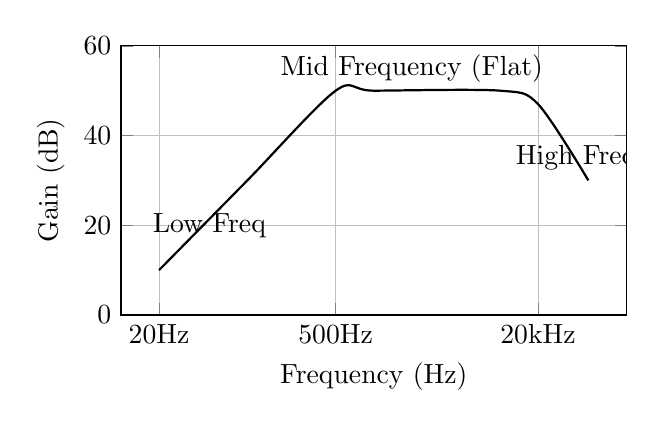
\begin{tikzpicture}
    \begin{semilogxaxis}[
        width=8cm, height=5cm,
        xlabel={Frequency (Hz)},
        ylabel={Gain (dB)},
        xmin=10, xmax=100000,
        ymin=0, ymax=60,
        xtick={20, 500, 20000},
        xticklabels={20Hz, 500Hz, 20kHz},
        grid=major
    ]
    \addplot[thick, smooth] coordinates {
        (20, 10) (100, 30) (500, 50) (1000, 50) (10000, 50) (20000, 47) (50000, 30)
    };
    
    \node at (axis cs: 50, 20) {Low Freq};
    \node at (axis cs: 2000, 55) {Mid Frequency (Flat)};
    \node at (axis cs: 40000, 35) {High Freq};
    
    \end{semilogxaxis}
\end{tikzpicture}
\end{center}

\begin{center}
\captionof{table}{Frequency Regions}
\begin{tabular}{|l|l|l|}
\hline
\textbf{Region} & \textbf{Frequency} & \textbf{Cause of Fall} \\ \hline
Low & 20Hz - 500Hz & Coupling Capacitors ($C_C$) high reactance \\ \hline
Mid & 500Hz - 20kHz & Constant Gain (Ideal operation) \\ \hline
High & > 20kHz & Transistor parasitic capacitances \\ \hline
\end{tabular}
\end{center}

\textbf{Two-Stage Effect:}
\begin{itemize}
    \item \textbf{Bandwidth}: Reduces compared to single stage ($BW_n = BW_1 \times \sqrt{2^{1/n}-1}$).
    \item \textbf{Gain}: Product of individual stage gains ($A_{total} = A_1 \times A_2$).
\end{itemize}
\end{solutionbox}
\begin{mnemonicbox}
LMH - Low frequencies by coupling caps, Mid frequencies flat, High frequencies by transistor caps.
\end{mnemonicbox}

\questionmarks{2}{a}{3}
\textbf{Briefly explain bandwidth and gain-bandwidth product of an amplifier.}

\begin{solutionbox}
\textbf{Bandwidth (BW):}
The range of frequencies over which the amplifier gain is at least 70.7\% (or -3dB) of its maximum value.
$BW = f_2 - f_1$

\textbf{Gain-Bandwidth Product (GBP):}
The product of the voltage gain and the bandwidth is constant for a given amplifier.
$GBP = A_v \times BW = \text{Constant}$

\begin{center}
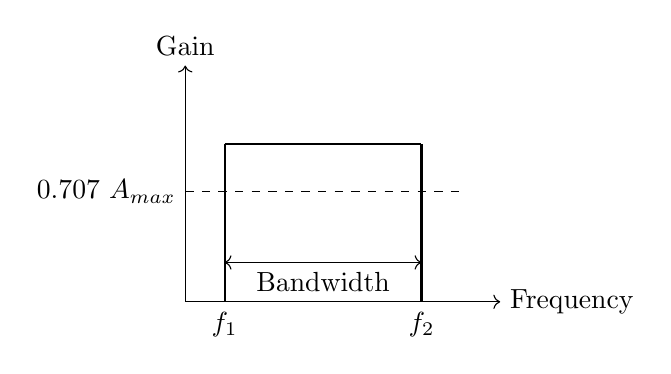
\begin{tikzpicture}
    \draw[->] (0,0) -- (4,0) node[right] {Frequency};
    \draw[->] (0,0) -- (0,3) node[above] {Gain};
    \draw[thick] (0.5,2) -- (3,2);
    \draw[thick] (0.5,2) -- (0.5,0) node[below] {$f_1$};
    \draw[thick] (3,2) -- (3,0) node[below] {$f_2$};
    \draw[dashed] (0,1.4) node[left]{0.707 $A_{max}$} -- (3.5,1.4);
    
    \draw[<->] (0.5, 0.5) -- (3, 0.5) node[midway, below] {Bandwidth};
\end{tikzpicture}
\end{center}
\end{solutionbox}
\begin{mnemonicbox}
BAND - Bandwidth And gain Never Drop together.
\end{mnemonicbox}

\questionmarks{2}{b}{4}
\textbf{Explain effects of emitter bypass capacitor and coupling capacitor on frequency response of an amplifier.}

\begin{solutionbox}
\textbf{Capacitor Effects:}

\begin{center}
\captionof{table}{Capacitors}
\begin{tabular}{|l|l|l|}
\hline
\textbf{Capacitor} & \textbf{Function} & \textbf{Effect} \\ \hline
Coupling ($C_C$) & Blocks DC, passes AC & Limits Low Frequency response (High reactance at low f) \\ \hline
Bypass ($C_E$) & Bypasses $R_E$ & Increases Mid-band gain. If removed, gain drops due to negative feedback. \\ \hline
\end{tabular}
\end{center}

\begin{center}
\begin{circuitikz}[scale=0.8]
    \draw (0,0) node[npn] (Q) {};
    \draw (Q.E) -- (0,-1) to[R, l=$R_E$] (0,-2.5) node[ground]{};
    \draw (0,-1) -- (1,-1) to[C, l=$C_E$] (1,-2.5) node[ground]{};
    \draw (Q.B) to[C, l=$C_C$] (-2,0) node[left]{Input};
\end{circuitikz}
\end{center}
\end{solutionbox}
\begin{mnemonicbox}
CELL - Coupling affects Extremely Low frequencies, bypass affects Low to high.
\end{mnemonicbox}

\questionmarks{2}{c}{7}
\textbf{Compare transformer coupled amplifier and RC coupled amplifier}

\begin{solutionbox}
\textbf{Comparison:}

\begin{center}
\captionof{table}{Transformer vs RC Coupled}
\begin{tabular}{|l|l|l|}
\hline
\textbf{Feature} & \textbf{Transformer Coupled} & \textbf{RC Coupled} \\ \hline
Coupling & Transformer & Resistor-Capacitor \\ \hline
Impedance Matching & Excellent & Poor \\ \hline
Frequency Response & Poor (Resonant peaks) & Good (Flat over wide range) \\ \hline
Efficiency & High & Low \\ \hline
Size/Weight & Bulky/Heavy & Small/Light \\ \hline
Cost & Expensive & Inexpensive \\ \hline
Application & Power Amplifiers & Voltage Amplifiers \\ \hline
\end{tabular}
\end{center}
\end{solutionbox}
\begin{mnemonicbox}
TRIP - Transformers are Robust for Impedance matching, Problematic for bandwidth.
\end{mnemonicbox}

\questionmarks{3}{a}{3}
\textbf{Describe the transistor used as a tuned amplifier.}

\begin{solutionbox}
\textbf{Tuned Amplifier:}
An amplifier that uses a parallel LC tank circuit as the collector load to amplify a specific narrow band of frequencies.

\begin{center}
\begin{circuitikz}[scale=0.9, transform shape]
    \draw (0,0) node[npn] (Q) {};
    \draw (Q.E) to[R, l=$R_E$] (0,-2) node[ground]{};
    \draw (Q.B) to[short, -o] (-1,0) node[left]{Input};
    
    % Tank Circuit
    \draw (Q.C) -- (0,1);
    \draw (-0.5,1) to[L, l=$L$] (-0.5,3);
    \draw (0.5,1) to[C, l=$C$] (0.5,3);
    \draw (-0.5,1) -- (0.5,1);
    \draw (-0.5,3) -- (0.5,3);
    \draw (0,3) node[vcc]{$+V_{CC}$};
    
    \draw (Q.C) to[C, l=$C_{out}$] (2,0) node[right]{Output};
\end{circuitikz}
\end{center}

\textbf{Key Components:}
\begin{itemize}
    \item \textbf{LC Tank}: Determines resonant frequency $f_r = \frac{1}{2\pi\sqrt{LC}}$.
    \item \textbf{High Q}: Provides high selectivity.
\end{itemize}

\textbf{Applications}: Radio and TV receivers (IF amplifiers).
\end{solutionbox}
\begin{mnemonicbox}
TUNE - Transistors Using Narrowband Elements for frequency selection.
\end{mnemonicbox}

\questionmarks{3}{b}{4}
\textbf{Explain in brief Direct coupled amplifier.}

\begin{solutionbox}
\textbf{Direct Coupled Amplifier:}
(See Q2(b) for diagram)
A multi-stage amplifier where the output of one stage is directly connected to the input of the next.

\textbf{Advantages:}
\begin{itemize}
    \item Low cost (no capacitors/transformers).
    \item Amplifies DC signals (0 Hz to high frequency).
\end{itemize}

\textbf{Disadvantages:}
\begin{itemize}
    \item Thermal drift issues (DC shift).
    \item Requires stable power supplies.
\end{itemize}
\end{solutionbox}
\begin{mnemonicbox}
DCAP - Direct Coupled Amplifier Passes all frequencies including DC.
\end{mnemonicbox}

\questionmarks{3}{c}{7}
\textbf{Describe the importance of h parameters in two port networks. Draw h-parameters circuit for CE amplifier.}

\begin{solutionbox}
\textbf{Importance of h-parameters:}
\begin{itemize}
    \item \textbf{Hybrid Nature}: Mix of impedance and admittance parameters.
    \item \textbf{Easy to Measure}: $h_{11}, h_{21}$ measured with output shorted; $h_{12}, h_{22}$ measured with input open.
    \item \textbf{Standard}: Manufacturers provide transistor specs in h-parameters.
\end{itemize}

\textbf{h-parameter Circuit for CE Amplifier:}

\begin{center}
\begin{circuitikz}[scale=1]
    \draw (0,0) node[left]{B} to[short, o-] (1,0) to[R, l=$h_{ie}$] (3,0) to[cV, l=$h_{re}V_{ce}$] (3,-2) to[short, -o] (0,-2) node[left]{E};
    
    \draw (5,0) to[cI, l=$h_{fe}I_b$, invert] (5,-2);
    \draw (7,0) to[R, l=$\frac{1}{h_{oe}}$] (7,-2); 
    \draw (5,0) to[short, -o] (8,0) node[right]{C};
    \draw (5,-2) to[short, -o] (8,-2) node[right]{E};
    
    \draw (3,0) -- (8,0);
    \draw (3,-2) -- (8,-2);
\end{circuitikz}
\end{center}

\textbf{Parameters:}
\begin{enumerate}
    \item $h_{ie}$: Input Impedance.
    \item $h_{re}$: Reverse Voltage Ratio.
    \item $h_{fe}$: Forward Current Gain ($\beta$).
    \item $h_{oe}$: Output Admittance.
\end{enumerate}
\end{solutionbox}
\begin{mnemonicbox}
HIRE - h-parameters Include Resistance and current gain Effectively.
\end{mnemonicbox}

\questionmarks{3}{a}{3}
\textbf{Compare transformer coupled amplifier and direct coupled amplifier.}

\begin{solutionbox}
\textbf{Comparison:}

\begin{center}
\captionof{table}{Comparison}
\begin{tabular}{|l|l|l|}
\hline
\textbf{Feature} & \textbf{Transformer Coupled} & \textbf{Direct Coupled} \\ \hline
Frequency Response & Bandpass (Poor Low/High) & DC to High Frequency \\ \hline
Cost & High & Low \\ \hline
Size & Bulky & Compact \\ \hline
Impedance Matching & Excellent & Poor \\ \hline
DC Isolation & Yes & No \\ \hline
\end{tabular}
\end{center}
\end{solutionbox}
\begin{mnemonicbox}
TDC - Transformers provide DC isolation, Direct provides Complete frequency range.
\end{mnemonicbox}

\questionmarks{3}{b}{4}
\textbf{Draw and Explain circuit diagram of common emitter amplifier.}

\begin{solutionbox}
\textbf{Common Emitter (CE) Amplifier:}

\begin{center}
\begin{circuitikz}[scale=0.9, transform shape]
    \draw (0,0) node[npn] (Q) {};
    \draw (Q.C) to[R, l=$R_C$] (0,2) -- (0,3) node[vcc]{$+V_{CC}$};
    \draw (Q.E) to[R, l=$R_E$] (0,-2) node[ground]{};
    \draw (Q.B) to[C, l=$C_{in}$] (-2,0) node[left]{Input};
    \draw (Q.C) to[C, l=$C_{out}$] (2,1) node[right]{Output};
    
    % Biasing (Voltage Divider simplified)
    \draw (Q.B) to[R, l=$R_2$] (-0.5,-2) node[ground]{}; 
    \draw (Q.B) to[R, l=$R_1$] (-0.5,3) -- (0,3);
\end{circuitikz}
\end{center}

\textbf{Explanation:}
\begin{itemize}
    \item \textbf{Input}: Applied to Base-Emitter.
    \item \textbf{Output}: Taken from Collector-Emitter.
    \item \textbf{Phase Shift}: 180$^\circ$ (Output is inverted).
    \item \textbf{Gain}: High voltage and current gain.
\end{itemize}
\end{solutionbox}
\begin{mnemonicbox}
CEA - Common Emitter Amplifies with signal inversion.
\end{mnemonicbox}

\questionmarks{3}{c}{7}
\textbf{Draw Transistor Two Port Network and describe h-parameters for it. Write down advantages of hybrid parameters.}

\begin{solutionbox}
\textbf{Two-Port Network:}
(See Q3(c) above for h-parameter model explanation).

\begin{center}
\begin{circuitikz}
    \draw (0,0) rectangle (4,2);
    \node at (2,1) {Two-Port Network};
    \draw (-1,1.5) to[short, i=$I_1$] (0,1.5);
    \draw (-1,0.5) to[short] (0,0.5);
    \draw (-1,1.5) to[open, v=$V_1$] (-1,0.5);
    
    \draw (5,1.5) to[short, i_=$I_2$] (4,1.5);
    \draw (5,0.5) to[short] (4,0.5);
    \draw (5,1.5) to[open, v^=$V_2$] (5,0.5);
\end{circuitikz}
\end{center}

\textbf{Equations:}
$V_1 = h_{11}I_1 + h_{12}V_2$ \\
$I_2 = h_{21}I_1 + h_{22}V_2$

\textbf{Advantages:}
\begin{itemize}
    \item Real numbers at audio frequencies.
    \item Easily measured.
    \item Suitable for circuit analysis.
\end{itemize}
\end{solutionbox}
\begin{mnemonicbox}
HAEM - Hybrid parameters Are Easily Measured.
\end{mnemonicbox}

\questionmarks{4}{a}{3}
\textbf{Explain Darlington pair and its applications.}

\begin{solutionbox}
\textbf{Darlington Pair:}
Two transistors connected in cascade ($CC-CC$) to behave like a single "super" transistor.

\begin{center}
\begin{circuitikz}
    \draw (0,0) node[npn] (Q1) {Q1};
    \draw (2,0) node[npn] (Q2) {Q2};
    \draw (Q1.C) -- (Q2.C) -- ++(0,0.5) node[vcc]{C};
    \draw (Q1.E) -- (Q2.B);
    \draw (Q1.B) -- ++(-0.5,0) node[left]{B};
    \draw (Q2.E) -- ++(0,-0.5) node[below]{E};
\end{circuitikz}
\end{center}

\textbf{Features:}
\begin{itemize}
    \item High Current Gain: $\beta \approx \beta_1 \beta_2$.
    \item High Input Impedance.
\end{itemize}
\textbf{Applications}: Power amplifiers, relay drivers, touch switches.
\end{solutionbox}
\begin{mnemonicbox}
DISH - Darlington Integrates Stages for High current gain.
\end{mnemonicbox}

\questionmarks{4}{b}{4}
\textbf{Describe the diode clamper circuit with necessary diagram.}

\begin{solutionbox}
\textbf{Diode Clamper:}
A circuit that shifts the DC level of a waveform.

\begin{center}
\begin{circuitikz}
    \draw (0,0) to[sinusoidal voltage source] (0,2) to[C, l=$C$] (2,2) -- (4,2) to[short, -o] (5,2) node[right]{Output};
    \draw (3,2) to[D*, l=$D$] (3,0);
    \draw (4,2) to[R, l=$R$] (4,0);
    \draw (0,0) -- (5,0) node[ground]{};
\end{circuitikz}
\end{center}

\textbf{Operation:} Capacitor charges to peak voltage, acting as a battery in series with the input signal, shifting it up or down.
\textbf{Application}: TV Receivers (DC restoration).
\end{solutionbox}
\begin{mnemonicbox}
CLAMP - Circuit Levels Are Modified Precisely.
\end{mnemonicbox}

\questionmarks{4}{c}{7}
\textbf{Explain the construction, working and applications of OLED.}

\begin{solutionbox}
\textbf{OLED (Organic Light Emitting Diode):}

\begin{center}
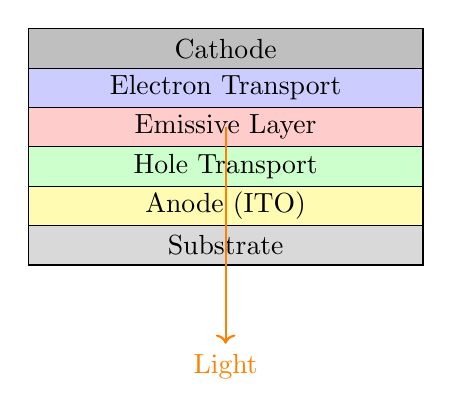
\begin{tikzpicture}
    % Layers
    \draw[thick] (0,0) rectangle (5,3);
    \draw[fill=gray!30] (0,0) rectangle (5,0.5) node[midway]{Substrate};
    \draw[fill=yellow!30] (0,0.5) rectangle (5,1) node[midway]{Anode (ITO)};
    \draw[fill=green!20] (0,1) rectangle (5,1.5) node[midway]{Hole Transport};
    \draw[fill=red!20] (0,1.5) rectangle (5,2) node[midway]{Emissive Layer};
    \draw[fill=blue!20] (0,2) rectangle (5,2.5) node[midway]{Electron Transport};
    \draw[fill=gray!50] (0,2.5) rectangle (5,3) node[midway]{Cathode};
    
    \draw[->, orange, thick] (2.5, 1.75) -- (2.5, -1) node[below]{Light};
\end{tikzpicture}
\end{center}

\textbf{Working}:
\begin{itemize}
    \item Charge carriers (holes and electrons) are injected from anode and cathode.
    \item They recombine in the emissive layer.
    \item Energy is released as light (Electroluminescence).
\end{itemize}

\textbf{Applications}: Curved screens, Flexible displays, High-end smartphones.
\end{solutionbox}
\begin{mnemonicbox}
OLED - Organic Layers Emit Directly.
\end{mnemonicbox}

\questionmarks{4}{a}{3}
\textbf{Explain Short note on LDR.}

\begin{solutionbox}
\textbf{LDR (Light Dependent Resistor):}
A photoresistor made of Cadmium Sulfide (CdS) whose resistance decreases when light shines on it.

\begin{center}
\begin{circuitikz}
    \draw (0,0) to[R, l=LDR] (2,0);
    \draw [->] (0.5, 1) -- (1, 0.5);
    \draw [->] (1, 1) -- (1.5, 0.5);
\end{circuitikz}
\end{center}

\textbf{Logic}: Light Energy creates electron-hole pairs $\rightarrow$ Conductivity increases $\rightarrow$ Resistance decreases.
\textbf{Use}: Street lights, alarms.
\end{solutionbox}
\begin{mnemonicbox}
LORD - Light Oppositely Reduces the Device's resistance.
\end{mnemonicbox}

\questionmarks{4}{b}{4}
\textbf{Describe the diode clipper circuit with necessary diagram.}

\begin{solutionbox}
\textbf{Diode Clipper:}
Removes parts of a signal.

\begin{center}
\begin{circuitikz}
    \draw (0,0) to[sinusoidal voltage source] (0,2) to[R, l=$R$] (2,2) -- (4,2) to[short, -o] (5,2) node[right]{Output};
    \draw (3,2) to[D*, l=$D$] (3,0) node[ground]{};
    \draw (0,0) -- (5,0);
\end{circuitikz}
\end{center}

\textbf{Positive Clipper}: Diode points down (removes positive).
\textbf{Negative Clipper}: Diode points up (removes negative).
\end{solutionbox}
\begin{mnemonicbox}
CLIP - Circuit Limits Input Peaks.
\end{mnemonicbox}

\questionmarks{4}{c}{7}
\textbf{Explain Half Wave and Full wave Voltage Doubler.}

\begin{solutionbox}
\textbf{Voltage Doubler:}
Produces DC voltage twice the peak AC input ($2V_m$).

\textbf{Half-Wave Doubler:}
\begin{center}
\begin{circuitikz}[scale=0.8]
    \draw (0,0) to[sinusoidal voltage source, l=$V_{in}$] (0,2) to[C, l=$C_1$] (2,2);
    \draw (2,2) to[D*, l=$D_1$] (2,0);
    \draw (2,2) to[D*, l=$D_2$] (4,2) to[C, l=$C_2$] (4,0);
    \draw (0,0) -- (4,0) node[ground]{};
    \node at (5,1) {$V_{out} \approx 2V_m$};
\end{circuitikz}
\end{center}

\textbf{Full-Wave Doubler:}
\begin{center}
\begin{circuitikz}[scale=0.8]
    \draw (0,2) to[sinusoidal voltage source] (0,0);
    \draw (0,2) to[D*, l=$D_1$] (2,2) to[C, l=$C_1$] (2,0);
    \draw (0,0) -- (2,0);
    \draw (0,2) to[C, l=$C_2$] (-2,2) to[D*, l=$D_2$] (-2,0) -- (0,0);
    % Simplified representation
\end{circuitikz}
\end{center}

\textbf{Explanation}: Capacitors charge in alternate cycles and their voltages sum up.
\end{solutionbox}
\begin{mnemonicbox}
DOUBLE - Diodes Organize Unidirectional Boost.
\end{mnemonicbox}

\questionmarks{5}{a}{3}
\textbf{Draw circuit diagram for +5 v Power Supply using its IC}

\begin{solutionbox}
\textbf{+5V Power Supply (7805):}

\begin{center}
\begin{circuitikz}
    \draw (0,0) node[draw, rectangle] (IC) {7805};
    \draw (IC.west) -- (-1,0) node[left]{Input (>7V)};
    \draw (IC.east) -- (1,0) node[right]{+5V};
    \draw (IC.south) -- (0,-1) node[ground]{};
    
    \draw (-0.5,0) to[C, l=$C_1$] (-0.5,-1) node[ground]{};
    \draw (0.5,0) to[C, l=$C_2$] (0.5,-1) node[ground]{};
\end{circuitikz}
\end{center}
\end{solutionbox}
\begin{mnemonicbox}
FIVE - Fixed IC Voltage Efficiently provided.
\end{mnemonicbox}

\questionmarks{5}{b}{4}
\textbf{Discuss load regulation and line regulation in reference to power supply.}

\begin{solutionbox}
\textbf{Regulation:} Keeping output voltage constant.

\begin{enumerate}
    \item \textbf{Line Regulation}: Ability to maintain constant $V_{out}$ when Input Voltage ($V_{in}$) changes.
    \[ \% \text{Reg} = \frac{\Delta V_{out}}{\Delta V_{in}} \times 100 \]
    \item \textbf{Load Regulation}: Ability to maintain constant $V_{out}$ when Load Current ($I_L$) changes.
    \[ \% \text{Reg} = \frac{V_{NL} - V_{FL}}{V_{FL}} \times 100 \]
\end{enumerate}
\end{solutionbox}
\begin{mnemonicbox}
LINE LOAD - Line Is Normal-input Efficiency, LOAD is Output Adjustment Defense.
\end{mnemonicbox}

\questionmarks{5}{c}{7}
\textbf{Explain adjustable voltage regulator using LM317 with circuit diagram.}

\begin{solutionbox}
\textbf{LM317 Adjustable Regulator:}

\begin{center}
\begin{circuitikz}
    \draw (0,0) node[draw, rectangle] (IC) {LM317};
    \node[left] at (IC.west) {IN};
    \node[right] at (IC.east) {OUT};
    \node[below] at (IC.south) {ADJ};
    
    \draw (IC.west) -- (-1,0) node[left]{$V_{in}$};
    \draw (IC.east) -- (2,0) node[right]{$V_{out}$};
    
    \draw (IC.east) to[R, l=$R_1 (240\Omega)$] (0.5,-1.5) -- (IC.south);
    \draw (0.5,-1.5) to[vR, l=$R_2$] (0.5,-3) node[ground]{};
    \draw (IC.east) to[C] (2,-3) node[ground]{};
\end{circuitikz}
\end{center}

\textbf{Formula}: $V_{out} = 1.25(1 + \frac{R_2}{R_1}) + I_{ADJ}R_2$.
\textbf{Use}: Bench power supplies.
\end{solutionbox}
\begin{mnemonicbox}
VARY - Voltage Adjustable Regulator Yields custom outputs.
\end{mnemonicbox}

\questionmarks{5}{a}{3}
\textbf{Draw circuit diagram for -15 v Power Supply using its IC}

\begin{solutionbox}
\textbf{-15V Power Supply (7915):}

\begin{center}
\begin{circuitikz}
    \draw (0,0) node[draw, rectangle] (IC) {7915};
    \draw (IC.west) -- (-1,0) node[left]{Input (-20V)};
    \draw (IC.east) -- (1,0) node[right]{-15V};
    \draw (IC.south) -- (0,-1) node[ground]{};
    
    \draw (-0.5,0) to[C] (-0.5,-1) node[ground]{};
    \draw (0.5,0) to[C] (0.5,-1) node[ground]{};
\end{circuitikz}
\end{center}
\textit{Note: 79xx series is for negative voltage.}
\end{solutionbox}
\begin{mnemonicbox}
NINE - Negative IC Needs Efficient filtering.
\end{mnemonicbox}

\questionmarks{5}{b}{4}
\textbf{Explain working of UPS.}

\begin{solutionbox}
\textbf{UPS (Uninterruptible Power Supply):}
Provides emergency power.

\begin{center}
\begin{tikzpicture}[node distance=2.5cm, auto]
    \node [gtu block] (Main) {Rectifier};
    \node [gtu block, right of=Main] (Bat) {Battery};
    \node [gtu block, right of=Bat] (Inv) {Inverter};
    
    \draw[gtu arrow] (Main) -- (Bat);
    \draw[gtu arrow] (Bat) -- (Inv);
    \draw[gtu arrow] (Inv) -- ++(1.5,0) node[right]{Output};
    
    \node [left of=Main, node distance=2cm] (AC) {AC In};
    \draw[gtu arrow] (AC) -- (Main);
\end{tikzpicture}
\end{center}

\textbf{Operation}:
1. Rectifier charges battery.
2. Inverter converts DC to AC for load.
3. If power fails, battery continues to supply inverter.
\end{solutionbox}
\begin{mnemonicbox}
UPBEAT - Uninterruptible Power Backup.
\end{mnemonicbox}

\questionmarks{5}{c}{7}
\textbf{Draw and explain SMPS block diagram with its advantages and disadvantages.}

\begin{solutionbox}
\textbf{SMPS (Switch Mode Power Supply):}

\begin{center}
\begin{tikzpicture}[node distance=2.5cm, auto]
    \node [gtu block] (Rect) {Rectifier};
    \node [gtu block, right of=Rect, align=center] (Switch) {High Freq\\Switch};
    \node [gtu block, right of=Switch, align=center] (Trans) {HF\\Transformer};
    \node [gtu block, right of=Trans, align=center] (Out) {Rectifier\\ \& Filter};
    
    \draw [gtu arrow] (Rect) -- (Switch);
    \draw [gtu arrow] (Switch) -- (Trans);
    \draw [gtu arrow] (Trans) -- (Out);
    
    \node [gtu block, below of=Switch, node distance=1.5cm] (Control) {PWM Control};
    \draw [gtu arrow] (Out) |- (Control);
    \draw [gtu arrow] (Control) -- (Switch);
\end{tikzpicture}
\end{center}

\textbf{Advantages}: High efficiency ($>80\%$), Compact size, Light weight.
\textbf{Disadvantages}: High noise (EMI), Complex circuit.
\end{solutionbox}
\begin{mnemonicbox}
SWITCH - Smaller Weight, Improved Thermal efficiency.
\end{mnemonicbox}

\end{document}
